\section{Anwendungen}

\subsection{Objektlageerkennung in Tiefendaten} 

\subsubsection{Ausgangslage}
In der Schmiede- und Giessereibranche ist das Handling der h"aufig
schweren und unhandlichen Werkst"ucke mittels Robotern eine grosse
Herausforderung. Eine der Grundvoraussetzungen ist dabei auch eine hohe
Flexibilit"at, um h"aufige Produktwechsel behandeln zu k"onnen. Ein
bekanntes Problem ist der sogenannte ``Griff-in-die-Kiste'', d.h. die
Entnahme eines bestimmten Gegenstandes aus einer mit mehreren chaotisch
angeordneten Objekten gef"ullten Kiste.

Die Dissertation \cite{Diss-Ledermann} von Thomas Ledermann
besch"aftigt sich u.a. mit der Entnahme von Getriebewellen f"ur eine
Ultraschallpr"ufung zur automatischen Qualit"atssicherung. Dabei stellt
sich zum Beispiel folgende Ausgangslage:

\begin{figure}[htbp]
	\centering
	\begin{minipage}{6cm}
		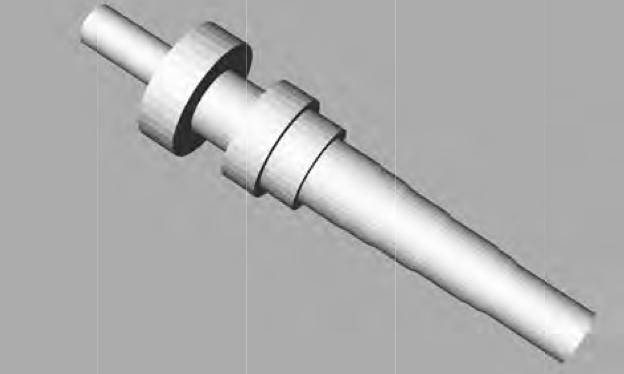
\includegraphics[width=5cm]{partikelschwarm/welle-cad}
	\end{minipage}
	\begin{minipage}{6cm}
		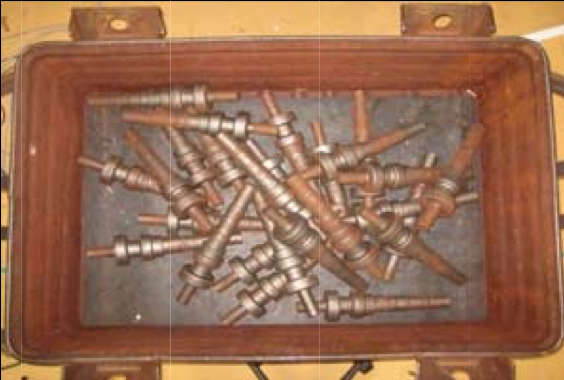
\includegraphics[width=5cm]{partikelschwarm/welle-kiste}
	\end{minipage}
	\caption{	Links: CAD-Modell einer Getriebewelle \\
				Rechts: Beispiel einer Kiste mit Getriebewellen zur Ultraschallpr"ufung}
	\label{Fig-Getriebewelle}
\end{figure}

Die Getriebewellen liegen ungeordnet in einer Kiste und m"ussen mit einem
Roboterarm entnommen werden. Die Aufgabe der Partikelschwarm-Optimierung
ist es, m"oglichst optimal die Position und Ausrichtung einer
Getriebewelle zu bestimmen, um diese mit einem Griff aufnehmen und
pr"ufen zu k"onnen.
Der Algorithmus muss so ausgestaltet werden, dass auch andere Objekte,
wie Hohlringe oder Geh"ausedeckel erkannt werden k"onnen. Die Werkst"ucke
liegen jedoch immer artenrein vor, d.h. es ist bekannt um welche
Teile es sich handelt (3D-CAD Daten sind bekannt), und es werden keine
verschiedenen Teile gemischt.

\subsubsection{Umsetzung}
Zur Erkennung der Objekte muss eine sog. Wissensbasis $W$ erstellt
werden. Diese besteht aus bekannten Merkmalen des zu erkennenden
Objekts. Gut auswertbar sind in erster Linie Merkmale, wie Kreise /
Ellipsen, Kantenz"uge, Ebenen, Volumenk"orper, Histogramme. Alle diese
Merkmale bis auf Histogramme schr"anken die Objektbeschreibung stark ein,
weil nicht alle Objekte "uber solche Merkmale verf"ugen. Die Wissensbasis
$W$ ist also eine Datenbank bestehend aus bekannten Histogrammen des zu
erkennenden Objekts.

F"ur die gegebenen Tiefendaten $T$ werden folgende Auswertungen gemacht,
um die Position eines Objekts m"oglichst genau bestimmen bzw. optimieren
zu k"onnen:

\textbf{Objektorientierung $R_i$}: Die Objektorientierung gibt an, mit
welchem Eintrag aus der Wissensbasis die Partikelposition verglichen
werden soll. Zur Bestimmung der Orientierung gibt es verschiedene
Ans"atze. Gegen"uber der Darstellung mittels Richtungskosinus oder
Quaternionen hat sich aufgrund der Einfachheit und der Anschaulichkeit
die in der Luftfahrt verbreitete Yaw-Pitch-Roll-Variante der Eulerwinkel
durchgesetzt.

\begin{figure}[htbp]
	\centering
	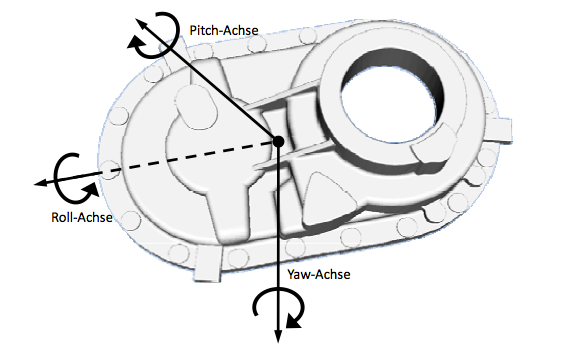
\includegraphics[width=6cm]{partikelschwarm/yaw-pitch-roll}
	\caption{Yaw-Pitch-Roll-Variante der Eulerwinkel}
	\label{Fig-Yaw-Pitch-Roll}
\end{figure}

\textbf{Objektposition $P_i$}: Die Objektposition gibt an, an welcher
Stelle der Tiefendaten der Vergleich stattfinden soll. Als Referenzpunkt
f"ur die Position ist der h"ochste Punkt des Objekts am besten geeignet,
weil dieser einfach aus den Tiefendaten extrahierbar ist. 

\textbf{Objektmerkmalsdaten $C_i$}: Die Objektmerkmalsdaten geben an,
welche Tiefendaten ausgehend von $P_i$ in die Auswertung einbezogen
werden sollen. S"amtliche Tiefenwerte, welche zur potentiellen Objektlage
geh"oren, m"ussen mittels einer geeigneten Segmentierung vom Hintergrund
getrennt werden. 


Die Fitnessfunktion ist abh"angig von all diesen Auswertungen:
\begin{equation}
	f(p_i) = f(R_i,P_i,C_i)
\end{equation}
Auf Basis dieser Werte wird die Fitnessfunktion "uber Vergleiche mit
bekannten Histogrammen aus der Wissensbasis $W$ berechnet.

\subsubsection{Resultate}
Der Partikelschwarm wird mit 100 Partikeln in lbest Topologie mit 30
Nachbarn realisiert. Bei 100 Iterationen wird innerhalb von 4 Sekunden
ein Resultat erreicht. In einer Kiste mit 50 Teilen wurden lediglich
4 Objektpositionen falsch erkannt, was einer Erkennungsrate von 92 \%
entspricht. Nach erneutem Scannen werden auch die falsch erkannten
Teile meist korrekt erkannt. Weitere Verbesserungen zur Verk"urzung der
Taktzeiten und zur gleichzeitigen Erkennung  mehrerer Objekte sind in
Planung und sollten gut realisierbar sein.

\subsection{Analyse neuronaler Netzwerke}
\index{neuronale Netzwerke!Analyse}
Ein weiteres Anwendungsgebiet, in welchem die Partikelschwarm-Optimierung
erfolgreich eingesetzt wird, ist die Analyse neuraler Netzwerke ,
u.a. in der Medizin. Eine "ubliche Anwendung ist bei der Diagnose
von Parkinson und Tremor zu finden. Dabei werden Bewegungsdaten
von einem Aktigraph-System (Messung der Bewegung, sowie der
Umgebungstemperatur und -Helligkeit) verarbeitet um zwischen
``normalen'' und von Krankheit verursachten Bewegungen zu
unterscheiden \cite{Shi-Appl}.

\subsection{Zucht von Mikroorganismen}
\index{Mikroorganismen}
Eine grosse Herausforderung in der Zucht von Mikroorganismen
ist die ideale Zusammensetzung der N"ahrstoffe. Die Verwendung
der Partikelschwarm-Optimierung ist in diesem Bereich weit
verbreitet. Gegen"uber klassischer Optimierungen hat die PSO komplett
andere Mischungen herausgebracht, welche sich als bis zu doppelt so
wirksam erwiesen haben \cite{Shi-Appl}.
